\documentclass[mathserif]{beamer}

\mode<presentation>
{
  %\usetheme{Hannover}
  \usetheme{Antibes}
  \usecolortheme{whale}
  \setbeamercovered{transparent}
}


\usepackage[encapsulated]{CJK}
\usepackage{ucs}
% one of bsmi, bkai, gbsn, gkai; see
% /usr/share/texmf-dist/tex/latex/cjk/texinput/UTF8/*.fd
\newcommand{\krtext}[1]{\begin{CJK}{UTF8}{mj}#1\end{CJK}}
\usepackage[utf8x]{inputenc}
\usepackage{listings}
\usepackage{verbatim}
\usepackage{graphicx}
\usepackage{amsmath,amssymb}


\newcommand{\vestigefunction}[3]{
  {
    \overbrace{\underbrace{{#1}}_{f(x)}}^{before} \;\;\;
    \overbrace{\underbrace{->}_{=}}^{{#2}} \;\;\;
    \overbrace{\underbrace{{#3}}_{y}}^{after}
  }
}

\title{Vestige}
\subtitle{A Tangible Interface for Learning Recursion and Functional Programming}
\author{Juan Diego Tascón Vidarte}
\institute{Konkuk University \\ HCI Lab}
\date{\today{}}

\AtBeginSection[] {
  \begin{frame} <beamer>{}
    \tableofcontents[currentsection]
  \end{frame}
}


\begin{document}

\begin{frame}
  \titlepage
\end{frame}

\begin{frame}{}
  \tableofcontents
\end{frame}

%*******************************************************************************
\section{Motivation}
%*******************************************************************************

\begin{frame}{Why Functional Programming?}
  \emph{Functional programming} is a programming style that relies
  mostly on mathematical functions and immutable data.
  \begin{block}{Properties}
    \begin{itemize}
    \item No arrays
    \item No loops
    \item No variable re-assignations
    \end{itemize}
  \end{block}
  \begin{block}{Benefits}
    \begin{itemize}
    \item Easy unitary tests
    \item Automatic concurrency
    \item Safe multi-threading
    \end{itemize}
  \end{block}
\end{frame}

\begin{frame}{Difficulties with Learning Recursion}
  \begin{itemize}
  \item Cognitive load theory: limited work memory~\footnote{The effect of
    dynamic copies model in teaching recursive prog.: Chen(1998)}.
  \item Base cases are hard to identify~\footnote{The case of bad cases: Haberman
    \& Averbuch(2002)}.
  \item It requires a good mathematical background~\footnote{The role of
    discrete math. and prog. in education: daRosa (2002)}.
  \item Computer scientist do not rationalize or use recursion to solve
    problems~\footnote{Do senior CS students capitalize on recursion?: Ginat(2004)}.
  \item One of the remedies introduced recursion in a gradual
    way~\footnote{A progressive approach to recursion: Velazquez(1999)}.
  \end{itemize}
\end{frame}

\begin{frame} {TUIs used to ease Learning}
  \begin{block}{Hypothesis}
    The use of physical materials per se could help on the
    process of learning
  \end{block}
  \begin{block}{Related work}
    \begin{itemize}
    \item Using material change the nature of the knowledge
      because perception and cognition are closely interlinked~\footnote{Do
        TUIs enhance learning: Marshall(2007)}.
    \item Children, people with learning disabilities and novices of any kind can
      be benefited by TUIs~\footnote{Extending TUIs for education: Zuckerman, Arida \& Resnick(2005)}.
    \item Several experiments had good results by using TUIs for learning:
      Tern~\footnote{Designing Tang. Prog. Lang. for classroom use: Horn \& Robert(2007)},
      Tangible bricks~\footnote{Tang. prog. bricks: making programming accessible to everyone McNerney(2002)}, etc.
    \end{itemize}
  \end{block}
\end{frame}

%*******************************************************************************
\section{Methodology}
%*******************************************************************************

\begin{frame}{Goal}
  Ease learning functional programming by means of an interactive
  interface based on a tangible block-world with augmented reality
  and software feedback.
  \vskip2ex
  \textsf{\bf Keywords:} \em{functional programming, tangible
    user-interface, block world, augmented reality, software
    feedback}
\end{frame}


\begin{frame}{Interaction}
  \begin{block} {What?}
    A block-world TUI with AR to provide feedback.
  \end{block}
  \begin{block} {How?}
    \begin{enumerate}
    \item Solve programming exercises by reorganizing a set of blocks.
    \item Blocks are guided and limited by gravity (imitating stacks).
    \item Multiple exercises in multiple scenarios (didactic phases).
    \item Transfer of training to Erlang (minimalist syntax).
    \end{enumerate}
  \end{block}
\end{frame}

\begin{frame}{Interface Elements}
  \begin{description}
  \item[Board:] The captured surface.
  \item[Blocks:] Any physical element above the board (Item, List,
    Switch).
  \item[Actions:] A blocks' movement (Pop, Push, Pop-Push, Create,
    Discard).
  \item[Scenes:] An arrangements of blocks.
  \item[Exercises:] Reverse, Join, Remove all, Compress, Insertion sort.
  \item[Feedback:] Messages and visual alerts.
  \item[Code suggestions:] Erlang code displayed.
  \end{description}
\end{frame}

\begin{frame}{Abstraction (1/3)}
  \begin{block}{Create}
    \begin{figure}
      \centering
      \subfigure{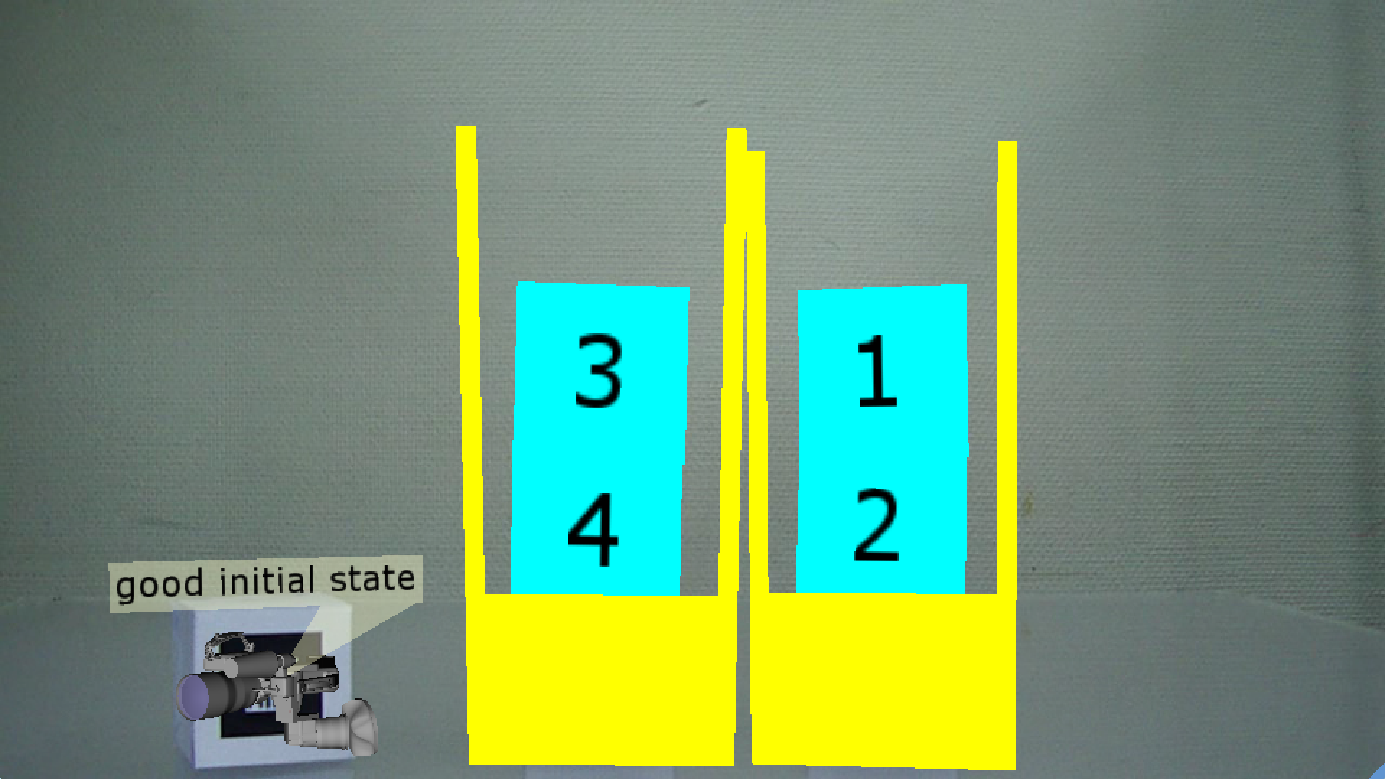
\includegraphics[scale=0.2]{img/actions/create1.pdf}}
      \subfigure{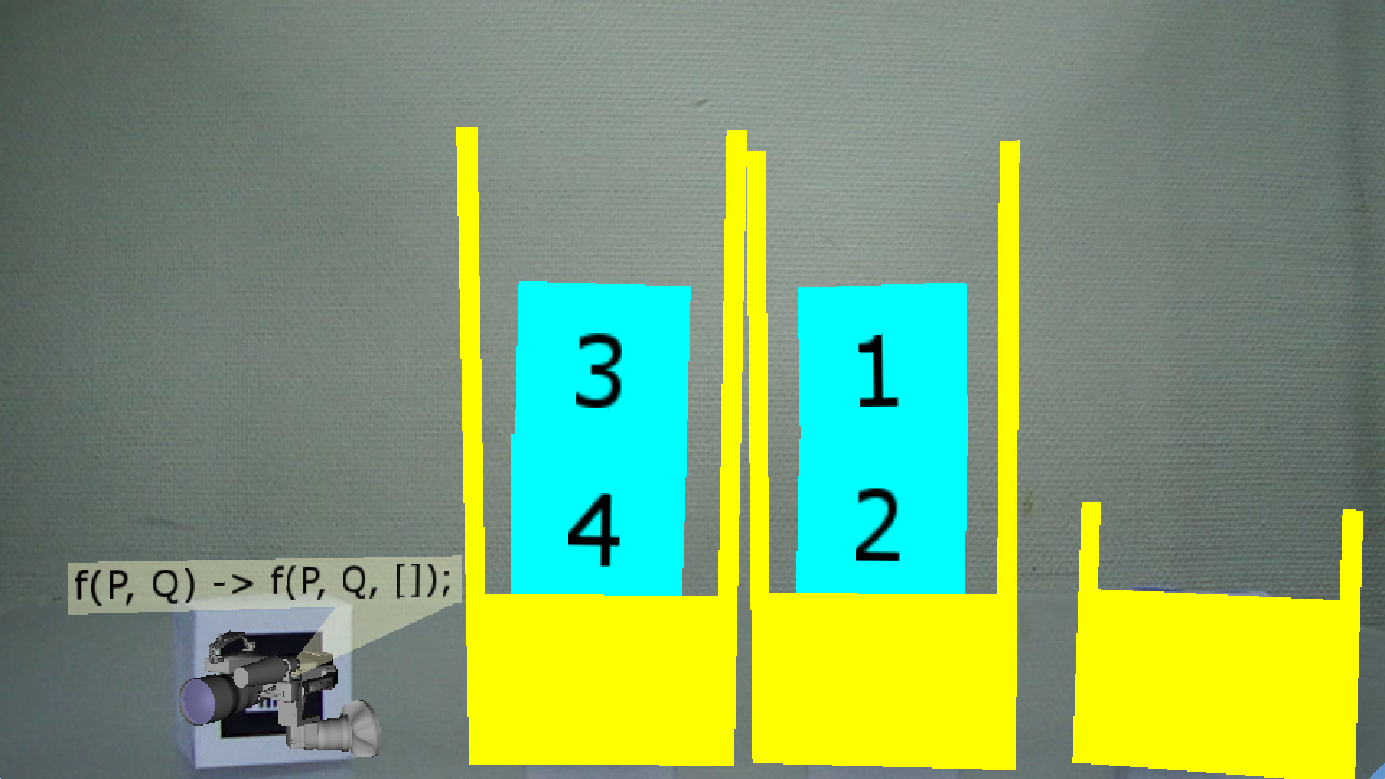
\includegraphics[scale=0.2]{img/actions/create2.pdf}}
    \end{figure}
    \centering{\small{ join(P,Q) $->$ join(P,Q,[]) }}
  \end{block}
\end{frame}
\begin{frame}{Abstraction (2/3)}
  \begin{block}{Pop-Push}
    \begin{figure}
      \centering
      \subfigure{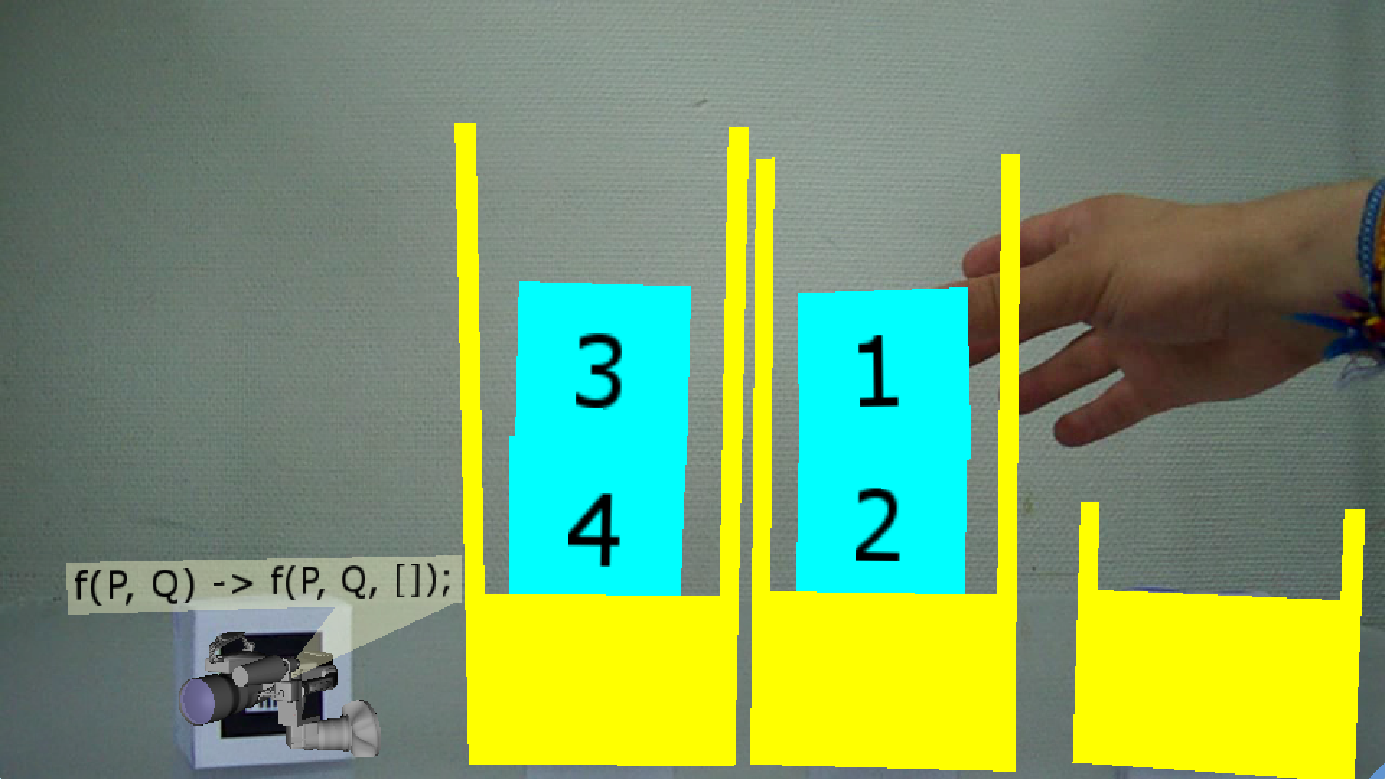
\includegraphics[scale=0.2]{img/actions/poppush1.pdf}}
      \subfigure{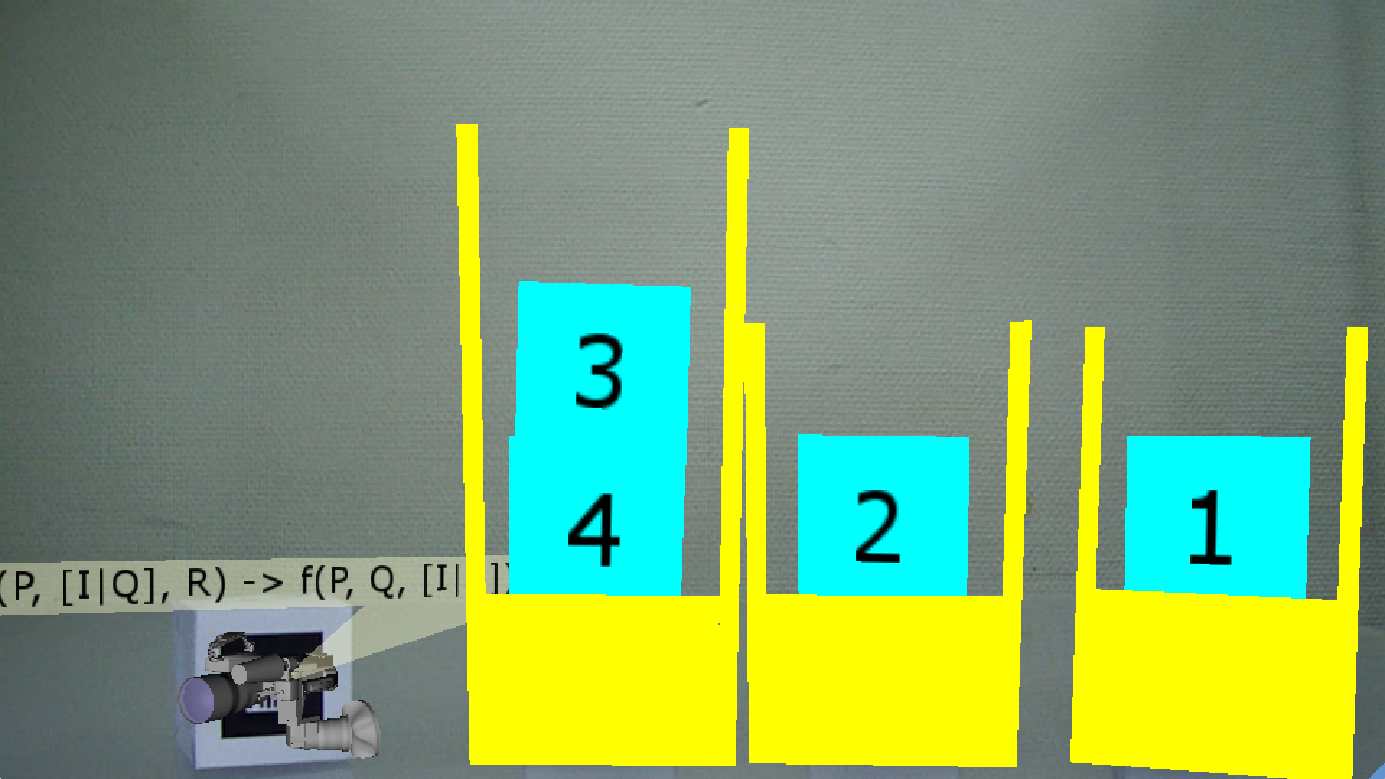
\includegraphics[scale=0.2]{img/actions/poppush2.pdf}}
    \end{figure}
    \centering{\small{ join(P,[I$|$Q],R) $->$ join(P,Q,[I$|$R]) }}
  \end{block}
\end{frame}
\begin{frame}{Abstraction (3/3)}
  \begin{block}{Discard}
    \begin{figure}
      \centering
      \subfigure{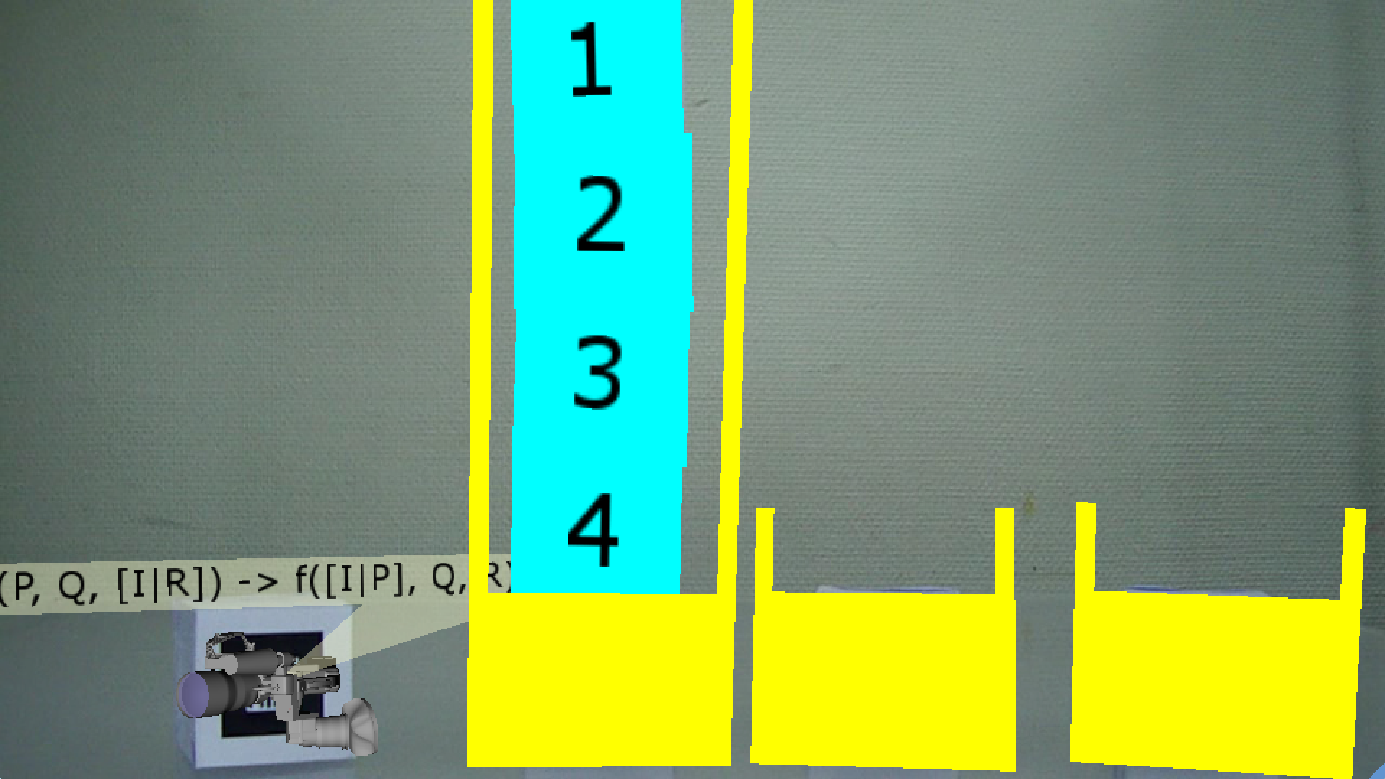
\includegraphics[scale=0.2]{img/actions/discard1.pdf}}
      \subfigure{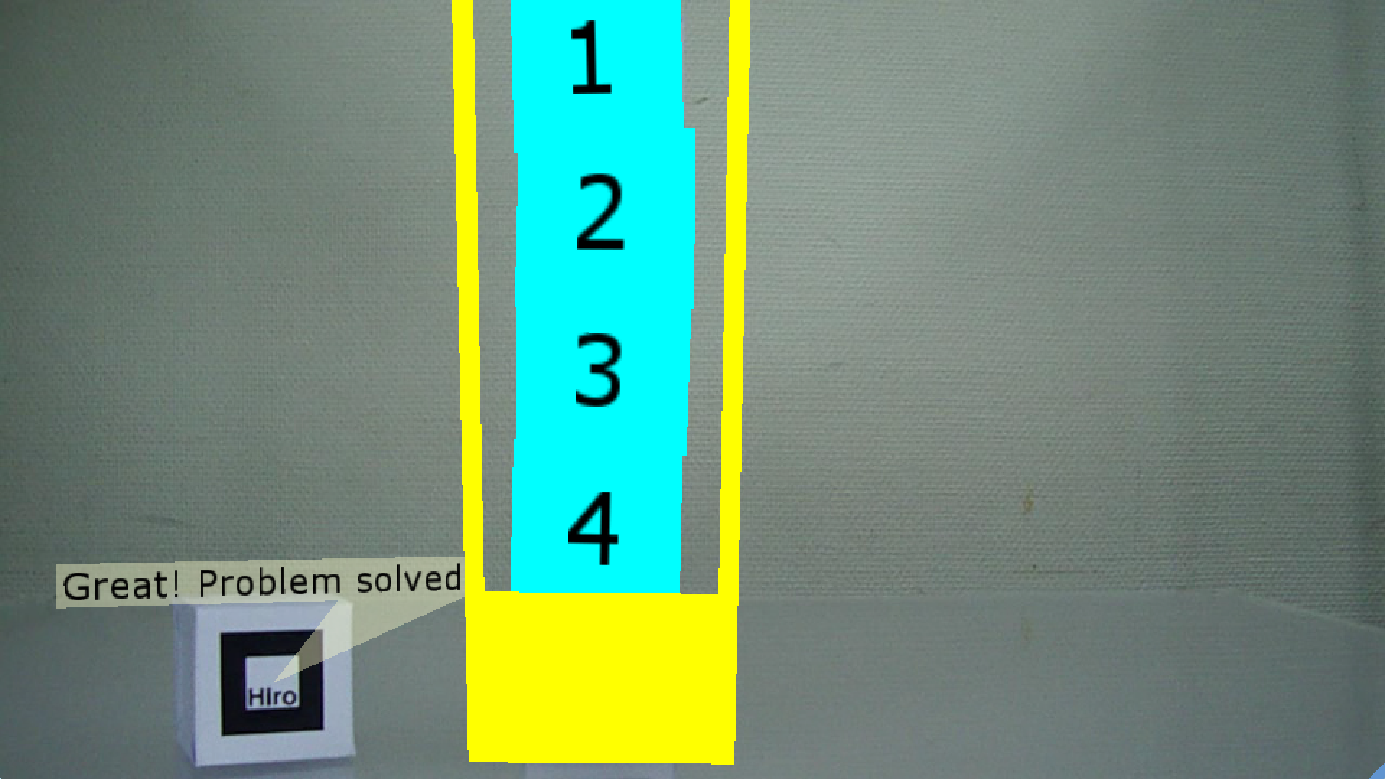
\includegraphics[scale=0.2]{img/actions/discard2.pdf}}
    \end{figure}
    \centering{\small{join(P,[],[]) $->$ P}}
  \end{block}
\end{frame}

\begin{frame}{Insertion Sort (1/2)}
  \begin{enumerate}
    \itemn{0} \small{\vestigef{isort(L)} {create} {isort(L,[],[])}}
    \itemn{3} \small{\vestigef{isort([I$|$L], D, [])} {poppush} {isort(L, D, [I])}}
    \itemn{4} \small{\vestigef{isort(X=[I$|$L], D, [AI$|$AL]) when (I $<$ AI)} {poppush} {isort(X, [AI$|$D], AL)}}
    \itemn{5} \small{\vestigef{isort([I$|$L], [], A=[\_$|$\_])} {poppush} {isort(L, [], [I$|$A])}}
  \end{enumerate}
\end{frame}

\begin{frame}{Insertion Sort (2/2)}
  \begin{enumerate}
    \itemn{6} \small{\vestigef{isort([I$|$L], D=[DI$|$\_], A=[\_$|$\_]) when (I $<$ DI)} {poppush} {isort(L, D, [I$|$A])}}
    \itemn{7} \small{\vestigef{isort(X=[I$|$L], [DI$|$DL], A=[\_$|$\_]) when (I $>$ DI)} {poppush}
      \newline\;\; {isort(X, DL, [DI$|$A])}}
    \itemn{2} \small{\vestigef{isort([], [DI$|$DL], A=[\_$|$\_])} {poppush} {isort([], DL, [DI$|$A])}}
    \itemn{1} \small{\vestigef{isort([], [], A)} {discard} {A}}
  \end{enumerate}
\end{frame}

\begin{frame}{Didactic Phases}
  \begin{enumerate}
  \item Concrete scenarios
  \item Generalization by introducing information hiding
  \item Abstraction by using variables
  \item Programming
  \end{enumerate}
\end{frame}

%*******************************************************************************
\section{Experiments}
%*******************************************************************************

\begin{frame}{Survey Results (1/2)}
  \begin{figure}
    \centering
    \subfigure{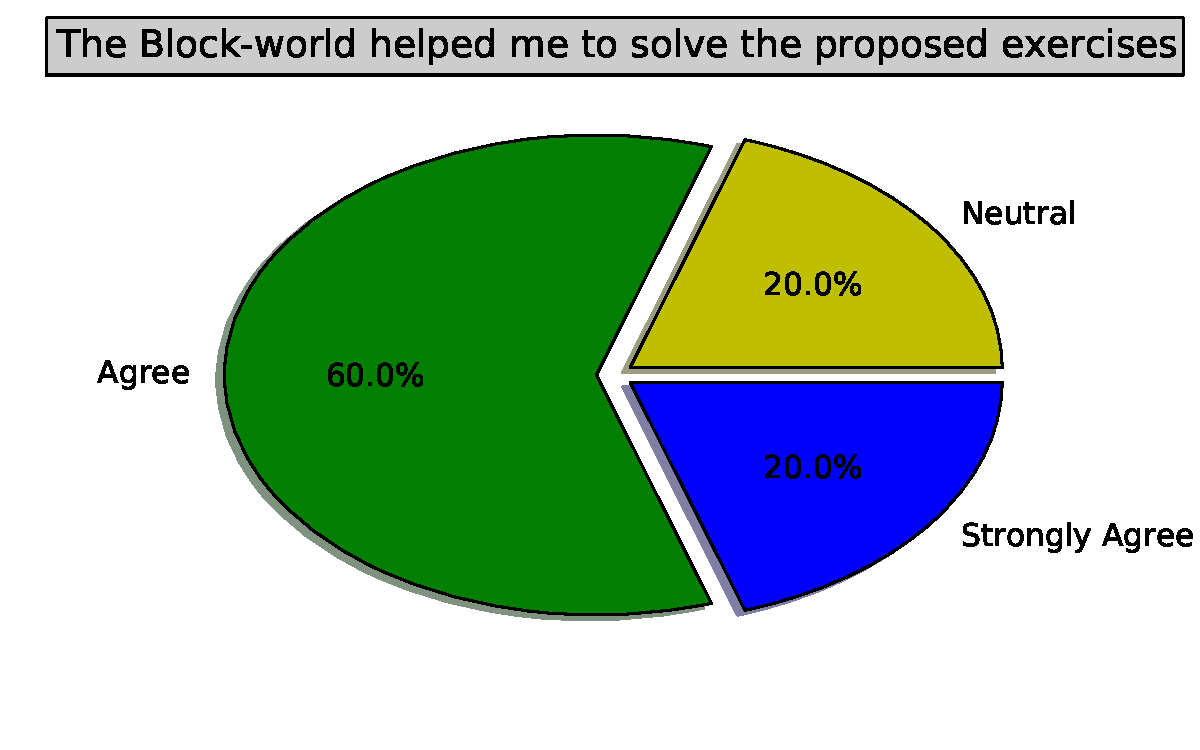
\includegraphics[scale=0.22]{img/survey/q5.pdf}}
    \subfigure{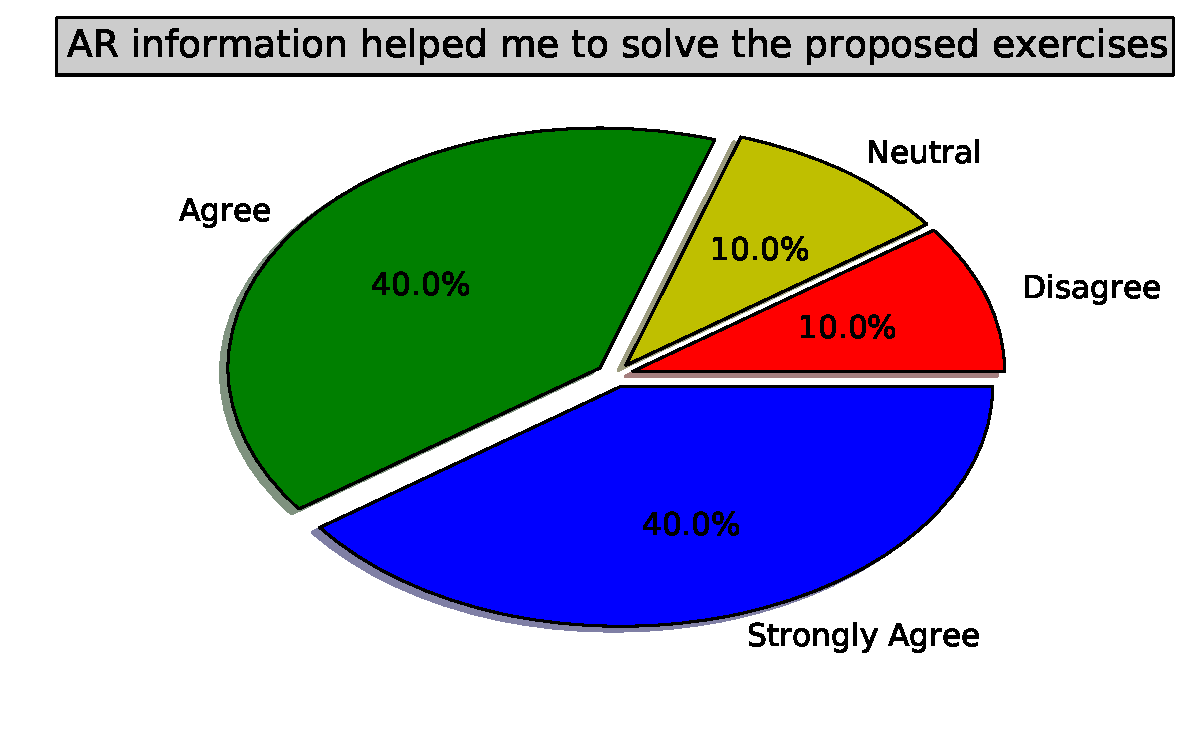
\includegraphics[scale=0.22]{img/survey/q6.pdf}}
    \subfigure{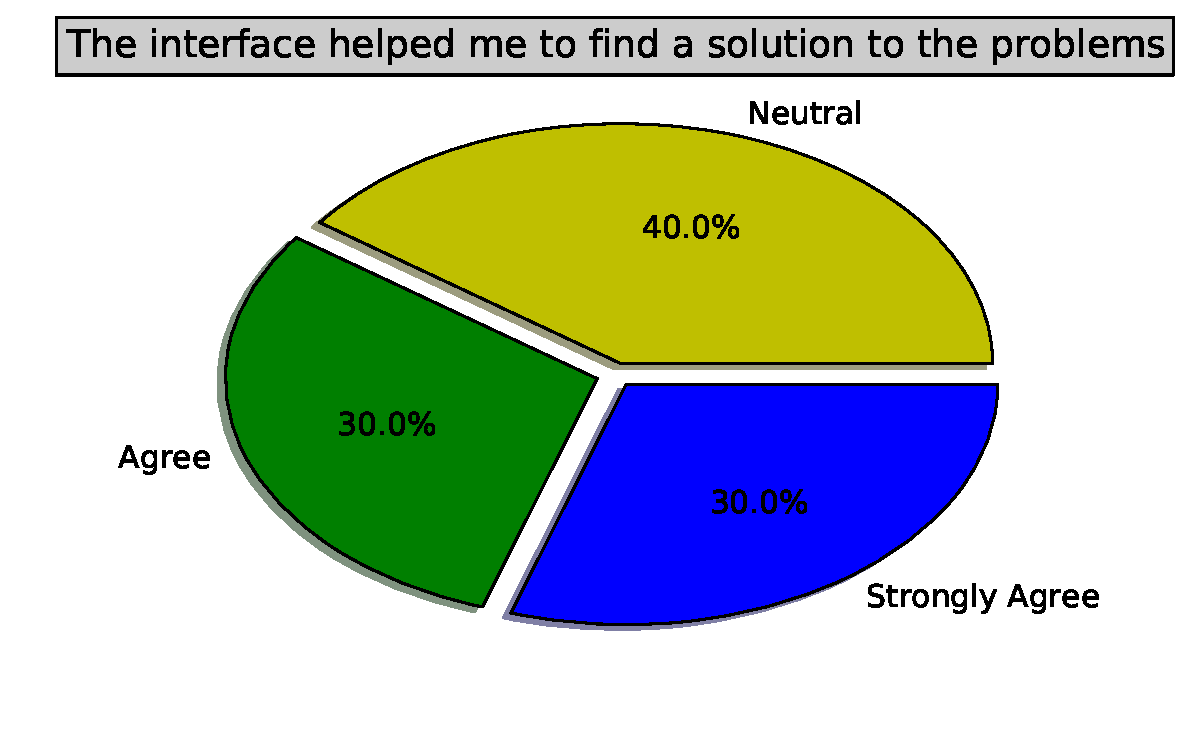
\includegraphics[scale=0.22]{img/survey/q7.pdf}}
    \caption{Interface related}
  \end{figure}
\end{frame}

\begin{frame}{Survey Results (2/2)}
  \begin{figure}
    \centering
    \subfigure{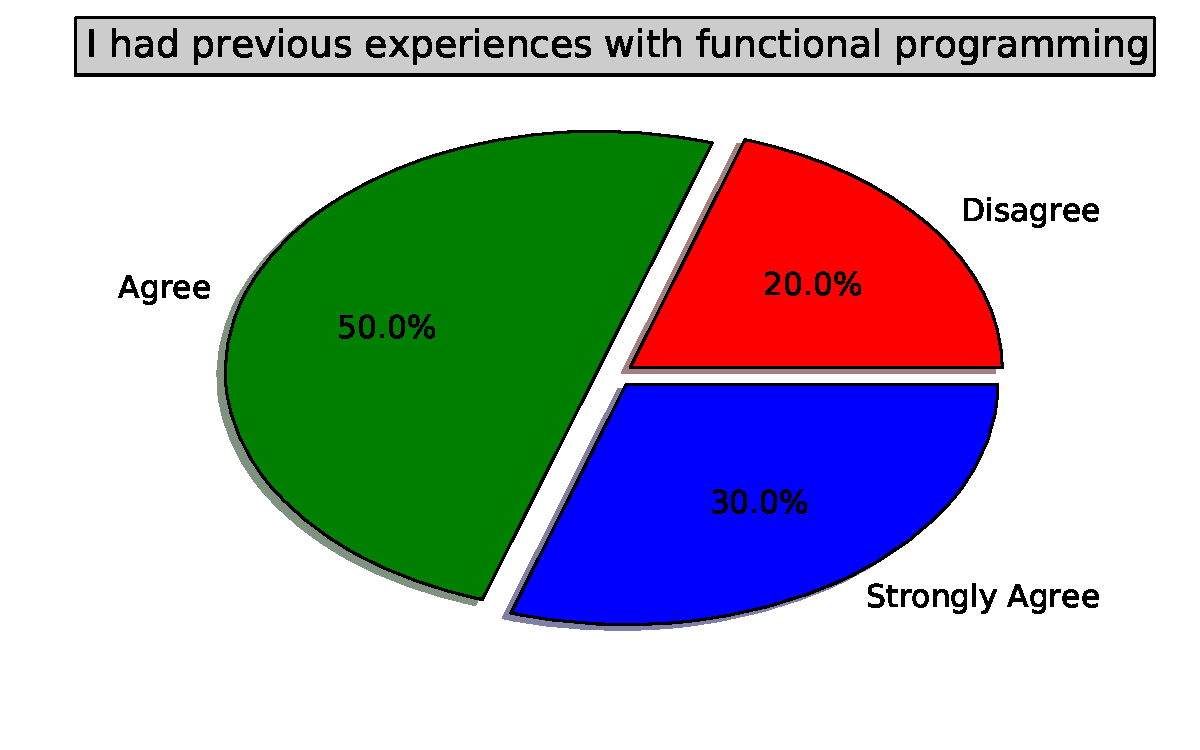
\includegraphics[scale=0.25]{img/survey/q2.pdf}}
    \subfigure{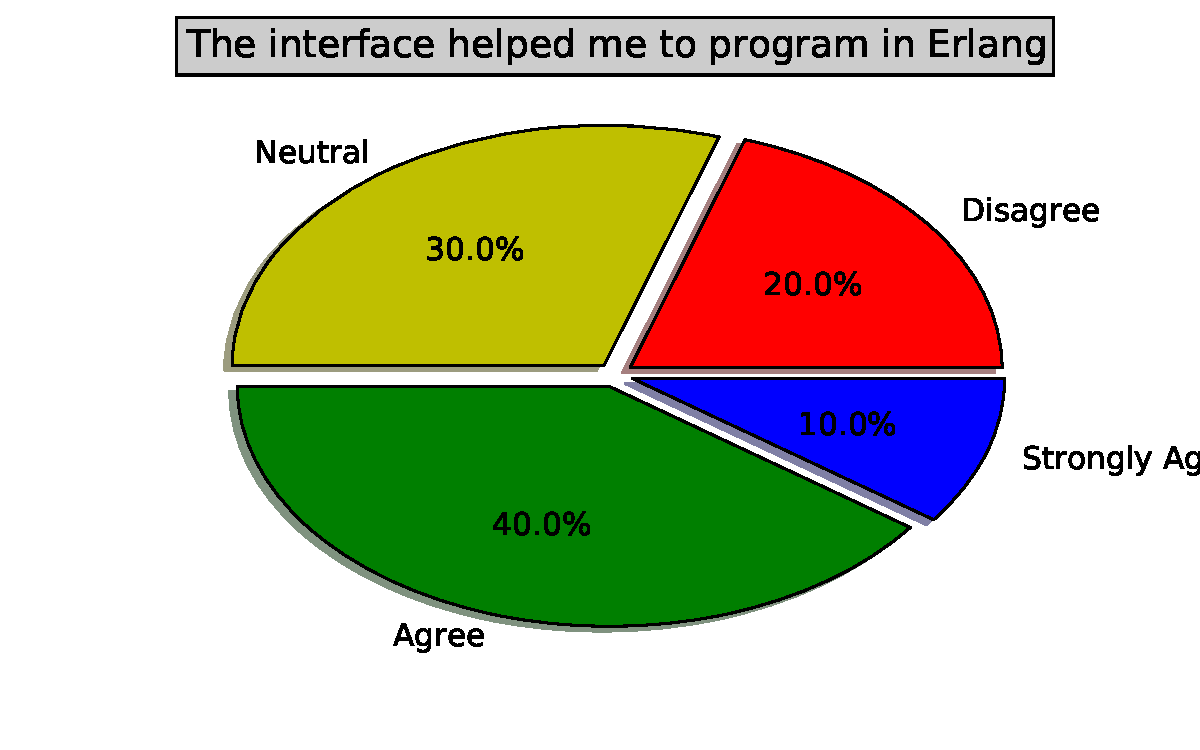
\includegraphics[scale=0.25]{img/survey/q8.pdf}}
    \caption{Erlang related}
  \end{figure}
\end{frame}

%*******************************************************************************
\section{Conclusions \& Future work}
%*******************************************************************************

\begin{frame}{Conclusions}
  \begin{block} {Conclusions}
    \begin{itemize}
    \item Tangible interface and methodology to ease learning recursion.
    \item Positive feedback after the initial experiment.
    \item Many students do not consider functional programming important.
    \end{itemize}
  \end{block}
  \begin{block} {Future work}
    \begin{itemize}
    \item Simulate a control stack.
    \item Implement more exercises (Hanoi towers, isort2, etc).
    \item Experiment during a class of functional programming.
    \end{itemize}
  \end{block}
\end{frame}

\begin{frame}{Summary}
  \begin{itemize}
  \item Why functional programming? (good benefits, recursion is hard)
  \item Why a tangible interface? (gravity, cognitive)
  \item How is the interface going to teach me recursion?
    (didactic phases, base cases, stack simulation)
  \end{itemize}
\end{frame}

\begin{frame}{Q/A?}
  \krtext{감사합니다}.
  \vskip3ex
  Q/A?
\end{frame}


\bibliographystyle{plain}
\bibliography{master}
\nocite{*}

\end{document}
